\documentclass[sigconf]{acmart}
%\settopmatter{printacmref=false} % Removes citation information below abstract
\renewcommand\footnotetextcopyrightpermission[1]{} % removes footnote with conference information in first column
\pagestyle{plain} % removes running headers

\usepackage{booktabs} % For formal tables
\usepackage{listings}
\usepackage{hyperref}
\hypersetup{
    colorlinks=true,
    linkcolor=blue,
    filecolor=magenta,      
    urlcolor=cyan,
}

\begin{document}
\title{Analyzing small world phenomenon and scale free network of python packages}

\author{Avadhoot Agasti}
\email{aagasti@indiana.edu}

\author{Abhishek Gupta}
\email{abhigupt@iu.edu}

\begin{abstract}

The \textit{small world} phenomenon is a very important and interesting concept which can be practically 
used in optimizing imports for programming languages like python, java etc. This will also help us understand
the network of the packages used by developers and classify them as scale free or random network. Further,
this analysis can be extended to any other programming language and understand the package network. The 
scope of this project is to focus on python based packages and navigate to all dependent packages to build
a network graph of these packages. Further, identify the important packages which could be like important
nodes in scale-free network.   
\end{abstract}

\keywords{scale-free, random networks, small-world, packages}

\maketitle

\section{Introduction} \label{intro}
When we try to install a python library, or rather when we use a python
library first thing that we need to do is to \textit{pip install} it.
Most of the times, a python library is dependent on another library. Our idea
 is to build a network or graph of the python library dependency. In this
 network, every library will be a node of the network and the dependency
 will form an edge.
 Such a graph can be queried to answer several questions like
\begin{itemize}
\item Which are the most core packages which are widely, directly or
undirectly, used in large number of other packages?
\item In which subject-area the new development is happening. We can pivot
this solution around the small number of packages which are included in large
 number of packages. For example, if networkX is being used by lot of new
 packages then we can say that there is lot of development happening in
 network science
\item What all packages will be impacted due to changes in a base package (e
.g. if we find a severe bug in networkX, what are the other packages which
can be potentially impacted due to the bug fix)
\end{itemize}
  
\section{Motivation} \label{intro}
There is not much work done around this topic and after reading the concepts
of network science it looks very interesting to find out how different module relate and how
these relations can be interpreted. This paper \textit{Power Laws in Software} \cite{louridas2008power} 
does analysis of power law distribution in a software application at class level and function level.
It did analysis of java, perl, c/c++ etc applications and did establish a pattern that 
these applications do follow power law distribution.

\begin{figure}[htbp]
\centering
\fbox{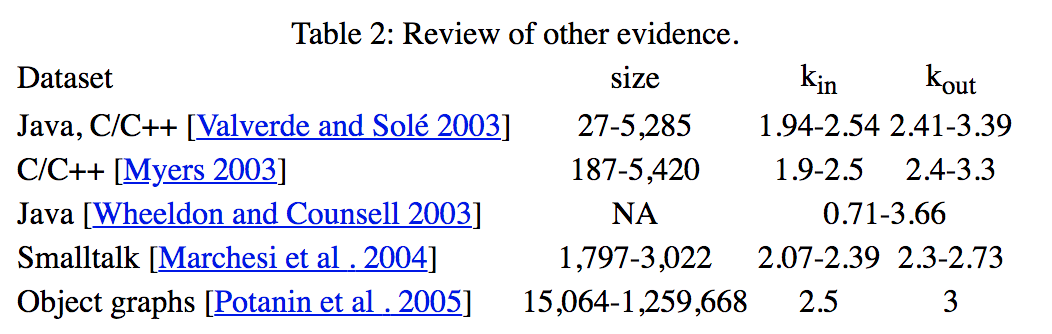
\includegraphics[width=\linewidth]{images/louridas2008power}}
\caption{Review of Languages}
\label{fig:louridas2008power}
\end{figure}

It depicts the size of datasets studied for this this analysis. However,
we couldn't find a paper or research which analyzes these patterns
 on all modules present in a given language.
Its very interesting problem to solve and find out how various python 
packages are dependent on each other and does it make sense 
to bundle some of the very common packages used along with base 
python distribution. It is interesting to understand the dependency structure 
but also to understand the community structure of these modules and 
what kind of network they form. Any other phenomenon exist when 
we analyze this graph. This analysis can be used to optimize the 
imports, remove cyclic dependencies between modules. Similar 
approach can be extended to other programming languages like java, ruby, perl etc.  
\section{Requirements} \label{req}
The goal of this analysis is
 \begin{itemize}
 \item to create a network graph of these dependencies
 \item understand the dependencies and important nodes
 \item identify if its a scale-free network
 \item identify any other properties depicted by this graph
 \item update the graph and build the graph as and when needed
 \end{itemize}
 At the end of this exercise we should be able to run this
 analysis on available python \cite{www-python-org} packages.
 Also, we need to understand and compute the other properties of the graph
 like average degree, average clustering co-efficient, average path length etc
 Also verify if the graph is \textit{scale free} or just a \textit{random} graph.  

\section{Technical Solution} \label{techsoln}

\subsection{Data Sources} \label{datasources}
 Our approach is to identify the dependent packages by looking
 at the dependencies using \textit{pip show} output. For example
 \begin{verbatim}
pip show networkx

Name: networkx

Version: 1.11

Summary: Python package for creating and 
manipulating graphs and networks

Home-page: http://networkx.github.io/

Author: NetworkX Developers

Author-email: networkx-discuss@googlegroups.com

License: BSD

Location: /Libs/anaconda/lib/python3.6/site-packages

Requires: decorator
 \end{verbatim}
 Looking at the above output we can clearly see that \textit{networkxx}
 depends on package \textit{decorator} and further package \textit{decorator}
 may be dependent on other package and so on. We continue to traverse
 we should be able to find all dependent packages till we reach code python
 libraries. Interestingly, there \textit{128k} python packages available
 \cite{www-python-org} which should give us a lot of data points for our
 analysis.

\subsection{Solution} \label{automation}
 Python app builds the graph using the installed modules in the local virtual
 environment. It runs \textit{pipdeptree}. The crawler module generates the
 dependency file with list of all recursive dependencies. Further, the parser recursively
 parses this dependency file and generates the directed graph as well as saves the
 graph in gml format. 
 
\begin{figure}[htbp]
\centering
\fbox{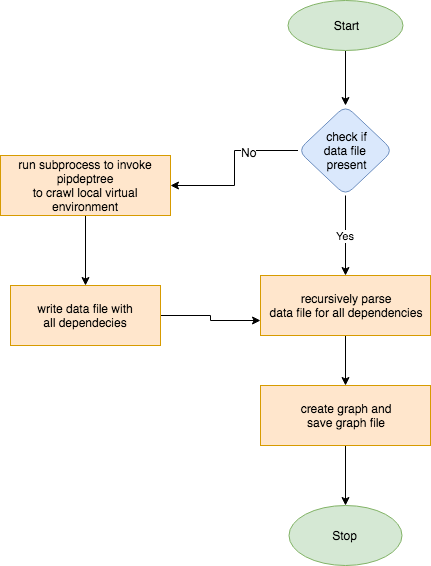
\includegraphics[width=\linewidth]{images/flowchart.png}}
\caption{Flow chart}
\label{fig:flowchart}
\end{figure}

Currently, this app relies on python modules installed in local environment only. 
Hence, we ended up installing bunch of python modules listed on pypi.org \cite{www-pypi}
to do this analysis. However, this work can be extended to crawl the python modules
listed on pypi.org \cite{www-pypi}. Installing all modules locally can be consume 
disk space, hence make sure you have enough disk space available if you plan to
install lot of modules and run the analysis. 
 Each package forms a node in the graph and each
 edge will represent the dependency with the next module. We should be able
 to plot this graph using \textit{networkx} module and represent the most important nodes
 which become the hubs to the network. Also, compute the degree and clustering 
 co-efficient for this graph. When you run the app, the app prints the number of vertices 
 and edges along with average in and out degree of the the graph.
 \begin{verbatim}
Type: DiGraph
Number of nodes: 242
Number of edges: 612
Average in degree:   2.5289
Average out degree:   2.5289
\end{verbatim}

\begin{figure}[htbp]
\centering
\fbox{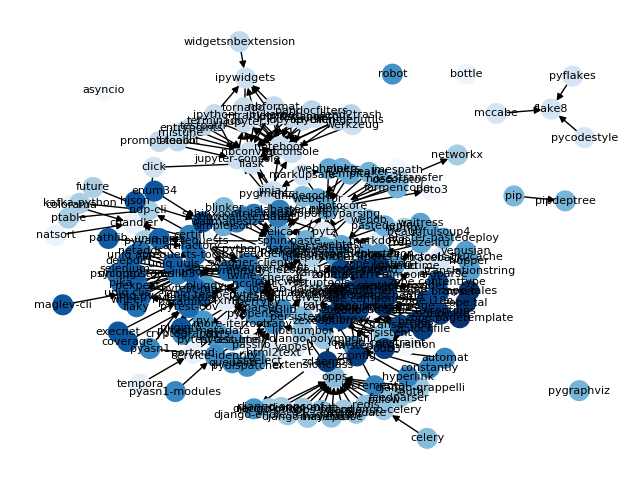
\includegraphics[width=\linewidth]{images/gengraph.png}}
\caption{Generated Output Graph}
\label{fig:gengraph}
\end{figure}
 
 Further, we study this graph to identify if the graph 
 follows the \textit{power law} distribution or it is a \textit{scale free} 
 network or its just a \textit{random} network. Also, see what kind of 
 community structure these module form.
 
\subsection{Technology} \label{tech}
We perform most of our coding in \textit{Python} and \textit{networkx} itself. 
We used \textit{Gephi} for visualizing the network.

\subsection{Challanges} \label{techchallanges}
During this exercise we ran into few technical challenges for example
to perform this analysis we have to install each python package locally
which could be really resource intensive specially in terms of disk space.
Also, while doing the analysis and loading the graph for 128k packages
could be memory and cpu intensive. To get around this problem we 
had to reduce the analysis to less number of python packages and keep
adding mode packages as we make progress. Further enhancements can be made
by running the crawler on pypi.org \cite{www-pypi}.
\section{Related Work} \label{relwork}
\begin {itemize}
\item
The project Pipedtree - \cite{www-pipdeptree} is command
line utility which allows user to see the installed packages in the form of
dependency tree. However, this utility is focused more on solving dependency
conflicts than the kind of analysis we propose to perform.

\item
Analysis of 30K Github projects \cite{www-takipi}.
The project was aimed to analyze the 30k different Java, Ruby and Javascript
projects on Github to understand the top libraries being used. While their
analysis was similar to what we plan to do, the approach was not network based.

\end {itemize}


%\input{similartechnologies}

%\input{conclusion}

%\end{document}  % This is where a 'short' article might terminate


\section{Acknowledgements}
 The authors thank Prof. YY Ahn for his technical guidance. The
 authors would also like to thank TAs of Network Science class for their valued
 support. 

\section{Repo} 
 All project and report document can be found at \href{https://github.com/avadhoot-agasti/netsci-project/blob/master/report/main.pdf}{github project}.

\nocite{*}
\bibliographystyle{unsrt}
\bibliography{references}

\end{document}
